\chapter{Variabili di processo per lavorazioni in asportazione di truciolo}
\label{chp:VarProcAsportazione}
GLi aspetti principali da considerare per tali lavorazioni sono:
\begin{itemize}
\item Finitura superficiale
\item lavorabilità,
\item forma, 
\item dimensioni, 
\item tolleranze,
\item tipo di lavorazione, 
\item macchine disponibili, 
\item valutazioni economiche
\end{itemize}

La prima decisione necessaria è la sequenza delle operazioni da eseguire.
Per ogni lavorazione bisogna scegliere velocità di taglio e avanzamento in funzione dei materiali del pezzo e utensile. Anche la fase della lavorazione 
va tenuta in conto, sgrossatura e finitura hanno due obbiettivi diversi 
e necessitano considerazioni diverse.

La finitura superficiale e le tolleranze dimensionali richieste vengono ottenute eseguendo un taglio di finitura con valori piccoli di avanzamento e profondità di passata.
Per cui in caso di oggetti \eng{near net-shape}, che possono presentare degli ossidi per via di lavorazioni a caldo precedenti, deve tenere in considerazione che un'operazione di finitura andrà a consumare maggiormente l'utensile: sapendo che il cambio utensile può essere svantaggioso in termini di finitura superficiale.

In una piccola officina il tempo non è un fattore eccessivamente importante.
Spesso ci si basa sull'esperienza dell'operatore per gestire la lavorazione
Diverso è il discorso per un'azienda ad alta produttività, in cui per tenere
basso il tempo ciclo di produzione è critico.
In questo caso, il \eng{set-up} può essere particolarmente problematico, 
allora alcuni enti hanno costituito col tempo, dei manuali da cui prendere
spunto per realizzare una lavorazione abbastanza rapidamente e senza eccessivo consumo dell'utensile. Alcuni esempi sono alle figure \ref{fig:Rel_VelTempDur} e \ref{fig:Rel_VelTempDur_NoFerr}. 

Ricordiamo che l'usura dell'utensile è determinata dalla temperatura raggiunta dall'utensile.
la temperatura, a sua volta, dipende dalla velocità di taglio.

Alla figura \ref{fig:Rel_VelTempDur} è mostrato un grafico che da una prima indicazione su come eseguire un tornitura per materiali ferrosi a diversa durezza. 

Nello specifico l'operazione di riferimento è una sgrossatura al tornio,
con taglienti che sono in acciai HSS oppure in carburo di titanio (non meglio specificati).
Il funzionamento è semplice: dato un lavorato di una certa durezza, si può ottenere una prima velocità di lavorazione sulla base di questo grafico.
la velocità dipende dal tipo di utensile sfruttato.

Altri grafici simili a \ref{fig:Rel_VelTempDur_NoFerr} vengono disposti per lavorazioni simili alla precedente ma su materiali non ferrosi, come indicati nella didascalia del grafico.

\begin{figure}
\centering
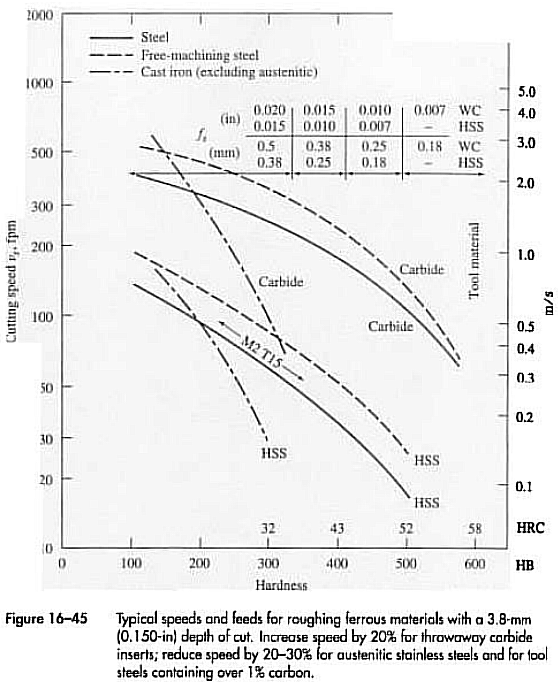
\includegraphics[width = \textwidth]{Rel_VelTempDur}
\caption{Relazione tra durezza del materiale lavorato, velocità della lavorazione e avanzamento dell'utensile.}
\label{fig:Rel_VelTempDur}
\end{figure}

\begin{figure}
\centering
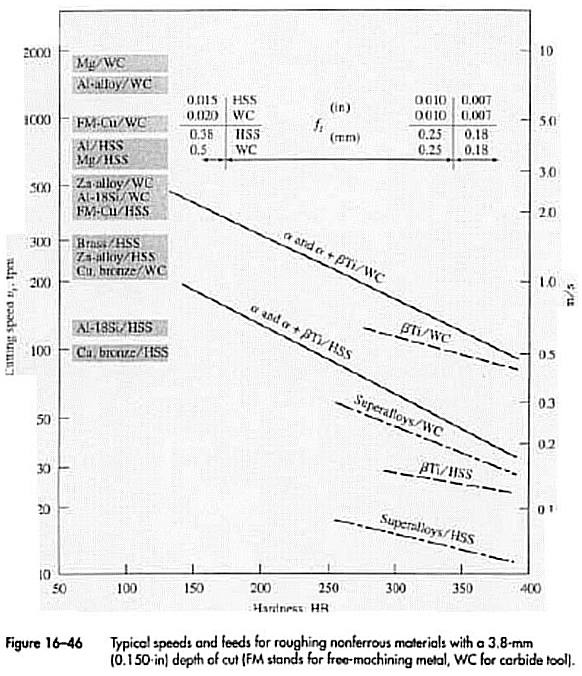
\includegraphics[width = \textwidth]{Rel_VelTempDur_NoFerr}
\caption{Prima velocità per materiali non ferrosi}
\label{fig:Rel_VelTempDur_NoFerr}
\end{figure}

I grafici \ref{fig:Rel_VelTempDur} e \ref{fig:Rel_VelTempDur_NoFerr} aiutano a scegliere i principali 3 parametri per le operazioni di sgrossatura.
Gli avanzamenti vanno scelti in funzione delle durezze dei materiali in cui si va a lavorare.
Si ha un'indicazione generica, un punto di partenza prudente, per la lavorazione. Le stime si basano sul portare la durata dell'utensile accettabile per circa 1-2 ore.
Tramite prove tecnologiche, si può accelerare la lavorazione se l'utensile arriva ad un tempo superiore alle 2 ore.
I riferimenti sono per un'operazione di tornitura. I manuali danno, in genere, i parametri di riferimento per altre operazioni come: fresatura, piallatura ecc\dots

\begin{figure}
\centering
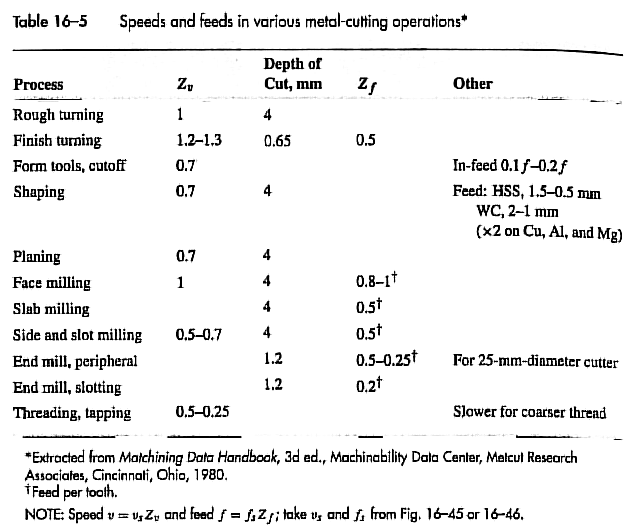
\includegraphics[width = \textwidth]{FattoriAltreLav}
\caption{Parametri modificatori per lavorazioni diverse da quelle di riferimento (tornitura in sgrossatura)}
\label{fig:FattoriAltreLav}
\end{figure}

Alla figura \ref{fig:FattoriAltreLav} sono riportati alcuni fattori di confronto rispetto alla lavorazione di riferimento. L'applicazione di tali coefficienti è riportata in descrizione alla figura.
Importanti sono: $Z_p$ e $Z_f$ sono dei coefficienti da moltiplicare ai riferimenti ottenuti dalla tornitura alle altre lavorazioni.
In generale valgono le seguenti:
\begin{align}
v &= Z_v * v_s\\
f &= Z_f * f_s\\
w &= \text{\eng{Depth of cut}} * w_s
\end{align}

La foratura con punta da trapano viene trattata a parte per via della sua natura. in generale si hanno dei valori piuttosto simbolici tipo $v = 0.7*v_s$ per il ferro e $v = 0.5*v_s$ per materiali non ferrosi.
Per esempio anche la profondità del foro gioca un ruolo importane nel controllo della temperatura.
Gli altri parametri dipendono dall'elica della punta, dal materiale della punta e dalla profondità come detto prima.
Anche la brocciatura ha dei parametri diversificati per cui viene descritta a parte.

Altri miglioramenti, in termini di velocità, si differenziano in base al materiale dell'utensile: per utensili ceramici si possono quasi raddoppiare le velocità di lavorazione (ovviamente da vedere nel caso specifico).

Non bisogna dimenticare anche altri aspetti tipo: rigidezza della macchina, il pezzo da ottenere, elementi di fissaggio, ecc\dots
Una macchina di alto livello riesce ad assorbire le vibrazioni non cedendole all'utensile: ottenendo un controllo migliore sulla lavorazione.

\section{Durata lavorazione e potenza macchina}
Una volta scelti i parametri di velocità e avanzamento di solito si stimano in sequenza:
\begin{enumerate}
\item la quantità di volume da rimuovere.
\item la velocità di rimozione del truciolo
\item Dai parametri precedenti si può stimare la durata della lavorazione come 
\begin{equation}
t_c = \frac{\overbrace{v_c}^{\text{velocità di taglio}}}{\underbrace{V_t}_{\text{volume rimosso}}}
\end{equation}
\item Si stimano energia specifica e successivamente la potenza richiesta dalla macchina.
\end{enumerate}

Si ricorda che la velocità di asportazione è data dalla velocità di taglio per la sezione trasversale del truciolo: spessore indeformato e profondità di passata.

\subsection{Esempio applicativo}
Si vuole allargare un foro in un getto in acciaio con un utensile in carburo. Il diametro iniziale è $D_i = 130\unit{\mm}$ a $D_f = 138\unit{mm}$. Si vuole suggerire velocità di taglio e avanzamento, profondità e potenza necessaria.

\missingfigure{Aggiungere i grafici di riferimento}

\subsection*{Soluzione}
Da manuale si ottengono: 
\begin{itemize}
\item $UTS$ del materiale: in questo caso $UTS = 485\unit{\MPa}$.
\item da cui si ricava $HB = 3*485*9.8=150\unit{\kg/\mm^2}$.
\end{itemize}
Allora possiamo stimare;
\begin{itemize}
\item Profondità di passata: $w = (138-130)/2 = 4\unit{\mm}$,
\item Dal grafico otteniamo: $v_s = 1.8\unit{\m/\s}$ che può essere aumentata del 20\% per via dell'utensile usa-e-getta al carburo da cui: $v_s = 1.8 * 1.2 = 2.16\unit{\m/\s}$
\end{itemize}
Siccome stiamo trattando una tornitura di interni:
\begin{itemize}
\item avanzamento: $f_s = 0.5\unit{\mm}$
\item siccome $Z_f = 1$ allora $f = 0.5\unit{\mm}$
\item Area trasversale truciolo: $A = f*w = 0.5*4 = 2\unit{\mm^2}$
\item Volume asportato: $V_t = A * v_s = 4320\unit{\mm^3/\s}$
\end{itemize}
Per calcolare la potenza:
\begin{itemize}
\item Dalla tabella: $E_1 = 2.1\unit{\W\s/\mm^2}$
\item Energia spesa: $E = E_1 * h^{-a}= 2.59\unit{\W\s/\mm^2}$
\item Da cui la potenza: $P = \frac{2.59 * 4320}{0.7} = 16\unit{\kW}$
\item la forza di taglio: $P_c = \frac{15956}{2.16} = 7.4\unit{\kN}$
\end{itemize}

%%%%%%%%%%%%%%%%%%%%%%%%%%%%%%%%%%%%%%%%%%%%%%%%%%%%%%%%%%%%%%%%%%%%%
% Macchine Utensili											       %
%%%%%%%%%%%%%%%%%%%%%%%%%%%%%%%%%%%%%%%%%%%%%%%%%%%%%%%%%%%%%%%%%%%%%
\chapter{Macchine Utensili}\label{chp:MacchineUtensili}
Spesso il cliente chiede delle macchine con delle specifiche particolari
in base alle lavorazioni che necessita.
In generale sono le dimensioni che differenziano le macchine.
Può capitare che ci siano delle necessità particolari per delle operazioni 
molto particolari.

Un caso particolare è rappresentato dalle macchine esapodi: presentano sei colonne che possono allungarsi e accorciarsi. Il vantaggio è che data la geometria impedisce alle colonne di flettere ma solo di porsi in trazione e compressione.
Ciò dovrebbe garantire altissima precisione e accuratezza nella lavorazione ma non hanno avuto grande successo per via del grande ingombro rispetto al volume lavorabile. Dunque poco adatte per una lavorazione industriale.

Si era già accennato lo sviluppo delle macchine a controllo numerico.
La diffusione di tali macchine è dovuta all'integrazione tra macchina e 
processore. La programmazione di queste macchine è in linguaggio ISO, in figura \ref{fig:ISO}.
Non è un linguaggio particolarmente comprensibile. Dunque gli sviluppi successivi hanno portato allo sviluppo del linguaggio APT, in figura \ref{fig:APT}.
Grazie all'evoluzione dei successivi sistemi CAD-CAM, si è sviluppato un metodo di programmazione più efficace. Si parte dal modello solido sviluppato tramite CAD, da cui vengono aggiunte delle geometrie semplici e poche istruzioni viene generato il linguaggio ISO da un compilatore.
Il risultato viene fornito alla macchina che potrà, dunque, lavorare.

\begin{figure}
\centering
\subfloat[][\emph{Esempio di programmazione in codice ISO}\label{fig:ISO}]
{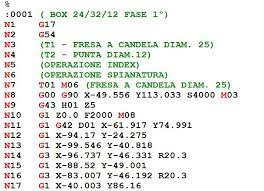
\includegraphics[width = 0.4\textwidth]{ISO}}\quad
\subfloat[][\emph{Esempio di programmazione in codice APT}\label{fig:APT}]
{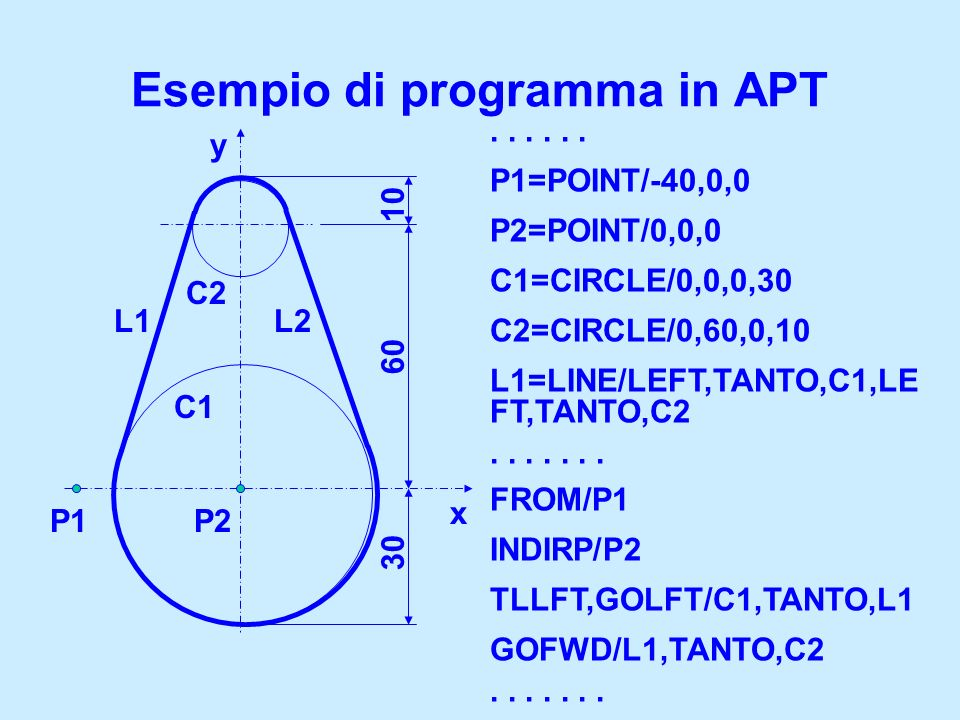
\includegraphics[width = 0.4\textwidth]{APT}}
\caption{Esempi di programmazione per macchine CNC}
\label{fig:CNC}
\end{figure}

Ulteriore problematica ed eventuale miglioramento delle macchine sta nella capacità di assorbire le vibrazioni. In generale le vibrazioni non sono ben volute durante queste lavorazioni per via del fatto che peggiorano la finitura. In più possono essere dannose per la componentistica abbordo macchina.

Passando ad un altro aspetto: ovvero la stabilità termica.
In generale una macchina provoca calore nella lavorazione. Dunque è necessario considerare l'eventuale dilatazione termica dovuta all'incremento della temperatura.
Allora sono state sviluppate delle tecniche di controllo adattativo: ovvero le macchine riescono a compensare delle variazioni durante la lavorazione, proprio come la dilatazione termica. 
Per esempio può essere rilevata la variazione dimensionale di un pezzo proprio per dilatazione termica, allora si può adattare la profondità dell'utensile per compensare tale variazione. 
Per questo scopo devono essere montati dei sensori abbordo macchina.
Eventualmente è necessario scegliere dei motori della macchina che possano compensare eventuali errori nel posizionamento come i motori a passo.

\subsection{Esempio di controllo numerico}
\missingfigure{Tabella confronto tra macchina tradizionale e \ac{FMS}}
Si evidenziano come i tempi di fissaggi sia la maggior parte di tempo persa durante una lavorazione per asportazione.

\section{Ottimizzazione delle lavorazione per asportazioni di truciolo}
L'obbiettivo dell'ottimizzazione ha come obbiettivo la massimizzazione dell'utile generato.
Possono sorgere altri fattori che cambino gli scopi dell'ottimizzazione, come arrivare a produrre un quantitativo di pezzi entro una certa data.

Premesse:
\begin{enumerate}
\item Si assume che la capacità della macchina sia adeguata alla lavorazione.
\item Il livello di finitura richiesto deve essere in linea col tipo di lavorazione che si va ad eseguire.
\item I fattori di costo devono essere noti.
\item Si assume che le costanti della formula di Taylor.
\begin{equation}
vT^n = cost.
\end{equation}
Le costanti note devono essere: $n$ e $cost.$
\end{enumerate}
Parametri che verranno considerati:
\begin{description}
\item[$t_c$] durata lavorazione pezzo [s],
\item[$R_t$] costo unitario [\$/min]
\item[$C_t$] costo di utensile [\$]
\item[$T_{ch}$] durata cambio utensile [s]
\item[$N_t$] Numero dei pezzi lavorati da un utensile
\item[$C_{tp}$] costo utensile per pezzo lavorato[\$]
\item[$C_{pr}$] costo per produrre un pezzo [\$]
\end{description}

Il costo della materia prima e i tempi di carico e scarico non influiscono sui costi di lavorazione.
Si va a valutare il costo dell'utensile per pezzo prodotto tramite la formula di Taylor descritta in \eqref{eqn:CostoUtensilePezzo}.
\begin{equation}
C_{tp} = \frac{1}{N_t} \left(T_{ch}R_t+C_t\right)
\label{eqn:CostoUtensilePezzo}
\end{equation}
a cui verranno sostituite le descrizioni dei vari parametri richiesti dalla stessa formula.
Per ottenere il costo di produzione complessivo bisogna aggiungere il costo di lavorazione:
\begin{equation}
C_{pr} = t_c R_t + \frac{1}{N_t} \left(T_{ch}R_t+C_t\right)
\end{equation}
Siccome la lavorazione dura:
\begin{equation}
t_c = \frac{l}{v}
\end{equation}
e il numero di pezzi prodotti:
\begin{equation}
N_t = \frac{\overbrace{t}^{\text{Durata utensile}}}{t_c}
\end{equation}
Allora:
\begin{equation}
C_{pr} = \frac{l}{v}R_t + \frac{t_c}{t}\left(t_{ch}R_t + C_t\right)
\end{equation}
La durata utensile è rappresentata da:
\begin{equation}
t = t_{ref}\left(\frac{C}{v}\right)^{1/n} \label{eqn:TUtensile}\end{equation}
Definitivamente si ottiene la formula di Taylor adattata per la lavorazione del caso:
\begin{equation}
C_{pr} = \frac{l}{v}R_t + \frac{l}{t_{ref}C^{1/n}}\left(t_{ch}+r_t\right)v^{\left(1-n\right)/n}\label{eqn:TaylorComp}
\end{equation}
per trovare il costo di produzione minimo derivo nella velocità la formula di Taylor opportunamente costruita \eqref{eqn:TaylorComp}:
\begin{equation}
\frac{dC_{pr}}{dv} = 0 = -\frac{l}{v}R_t + \frac{1-n}{n}\frac{l}{t_{ref}C^{1/n}} \left(t_{ch}R_t + C_t \right)v^{\left(1-2n\right)/n}
\label{eqn:MinCost}
\end{equation}
Si può esprimere a partire da \eqref{eqn:TaylorComp} un'espressione della velocità minima della lavorazione per garantire il raggiungimento del target della \eqref{eqn:MinCost}:
\begin{equation}
v_{c,min}  = C \left[\frac{n}{1-n}\left(\frac{t_{ref}R_t}{t_{ch}R-t + C_t}\right)\right]
\label{eqn:MinSpeed}
\end{equation}
La velocità di taglio cresce al crescere di $n$, il quale dipende dal materiale dell'utensile: più pregiato più $n\nearrow$. Inoltre la velocità di taglio ottimale cresce col crescere di $R_t$: il quale dipende dai vari costi per la gestione dell'azienda, costo operatore, ammortamento macchina ecc\dots

\begin{figure}
\centering
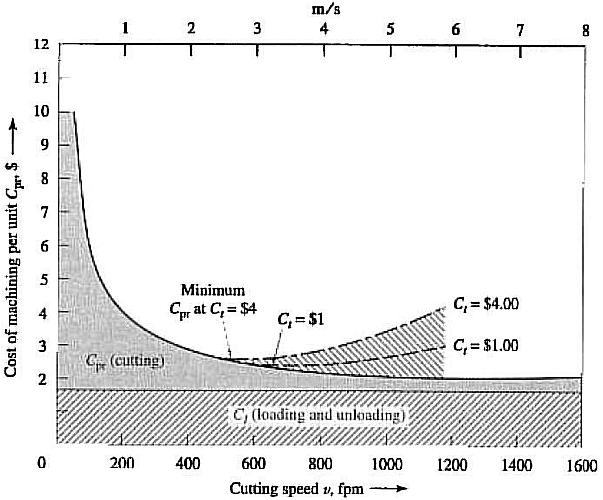
\includegraphics[width = \textwidth]{OttimizzazioneSpeed}
\caption{Rappresentazione della funzione \eqref{eqn:TaylorComp}}
\label{fig:OttimSPeedCost}
\end{figure}

